\subsection{Patients}

Three hand amputees, patients of the INAIL Centro Protesi in Vigorso
di Budrio, Bologna, Italy, joined the experiment.

The first subject is a male, aged 63, trans-radial one-third proximal,
amputated in 1963. He is a pioneer of myoelectric prostheses, having
started out using them in the Sixties. The second subject is male,
aged 56, trans-radial one-third distal, amputated in 1972; he also
started using myoelectric prostheses very early, actually in 1974. The
third subject is male again, aged 25, trans-carpal, amputated in 2007;
he was in the process of learning how to use a standard myoelectric
prosthesis at the time of writing.

A set of three patients is obviously not sufficient to gather
statistics about the applicability of our method, but we are lucky
enough that they present a rather wide variety of operations and
conditions. In particular, subject $1$ has about $9$cm left of his
left forearm, subject $2$ has some $20$cm, and subject $3$, a
trans-carpal amputee, has the whole forearm plus some of the carpus
(Figure \ref{fig:stumps} shows the subjects' stumps). Moreover,
subjects $1$ and $2$ were amputated a very long time ago, although
they have been using myodevices since then, whereas subject $3$ is
freshly operated and is just starting to learn. Lastly, subject $3$ is
rather young as opposed to the other subjects.

\begin{figure*}[!ht] \centering
  \begin{tabular}{ccc}
    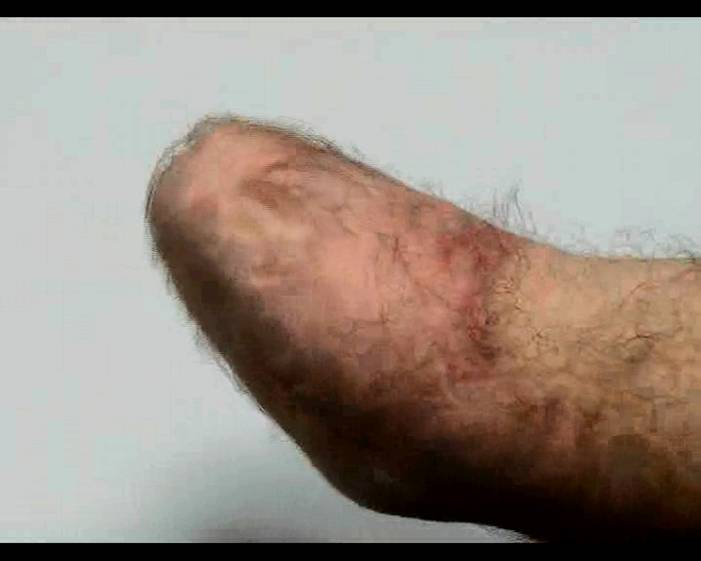
\includegraphics[width=0.3\textwidth]{figs/stump_1} &
    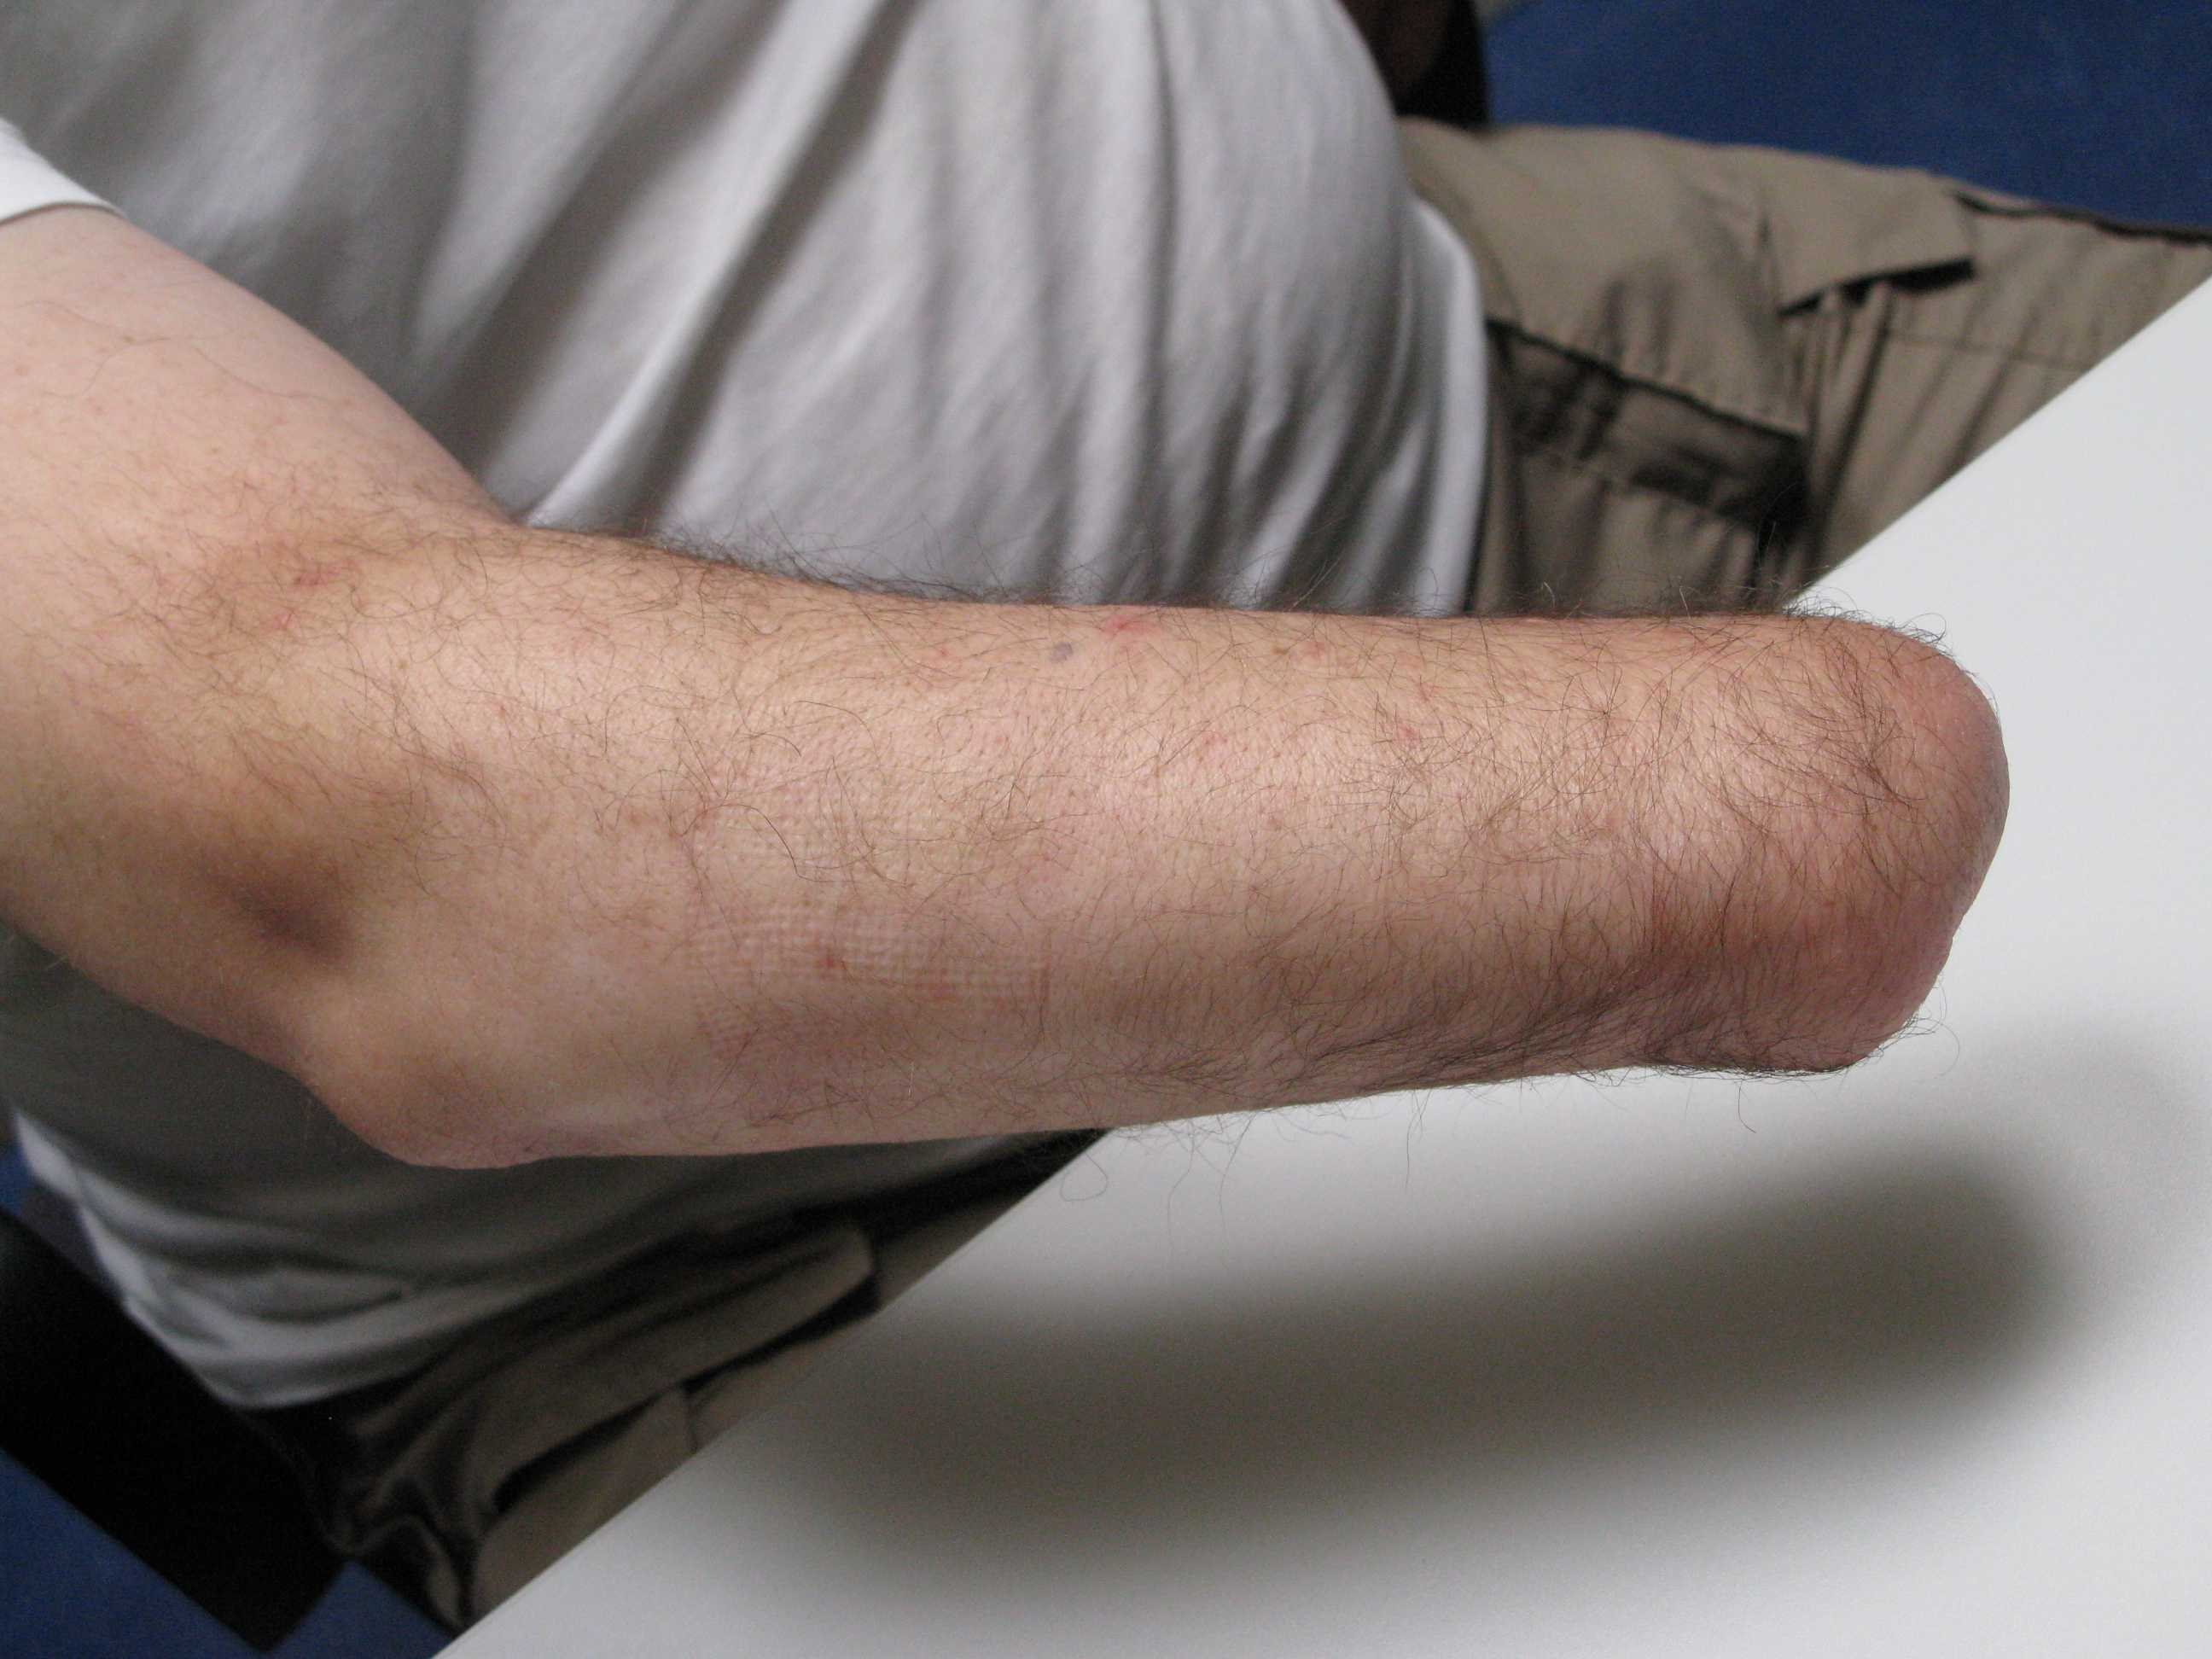
\includegraphics[width=0.3\textwidth]{figs/stump_2} &
    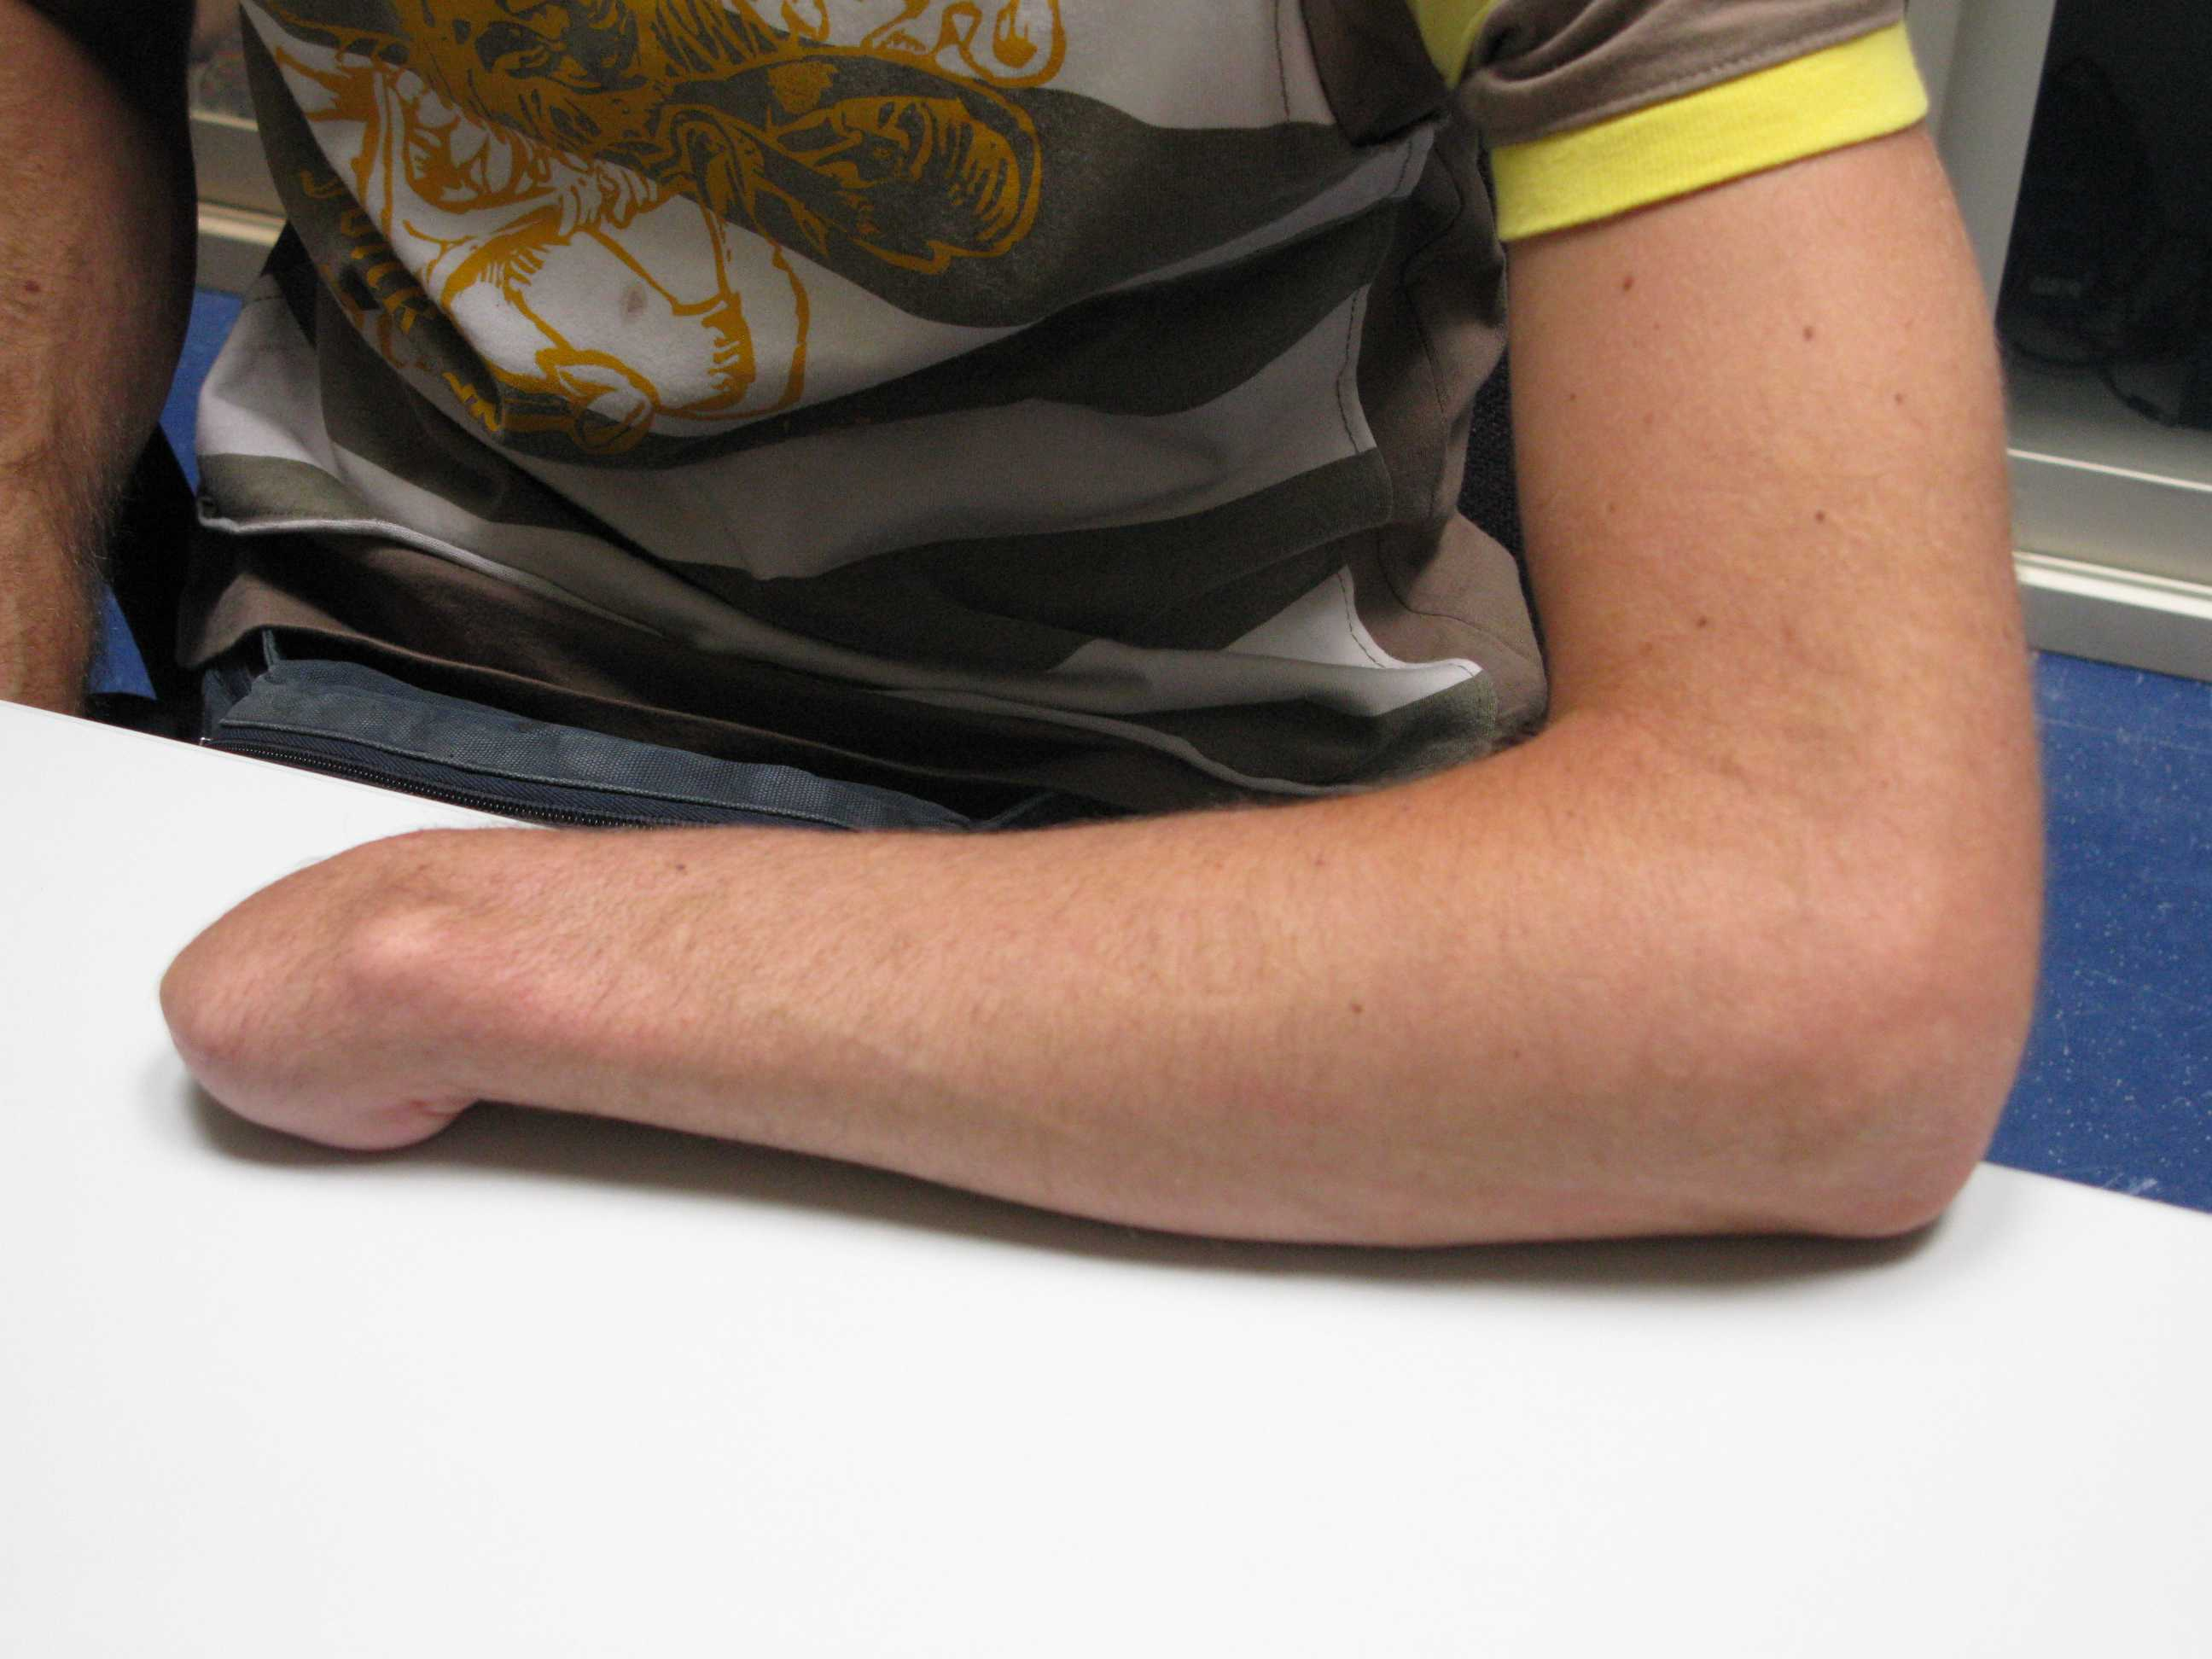
\includegraphics[width=0.3\textwidth]{figs/stump_3} \\
    subject $1$ & subject $2$ & subject $3$ \\
  \end{tabular}
  \caption{the subjects' stumps. Subject $1$ has a trans-radial
    one-third proximal amputation, leaving about $9$cms. of forearm in his
    stump; subject $2$ is trans-radial one-third distal, left with some
    $20$cms. of forearm; and subject $3$ is trans-carpal, still having his
    full forearm.}
  \label{fig:stumps}
\end{figure*}

\subsection{Setup}

We placed on each subject's stump $5$ surface EMG electrodes without
searching for the best anatomical position, but rather in a standard
way for all, around the stump, near the elbow (for subject $1$ this
was actually the only possible choice!) and at uniform angles from one
another, in such a way to "wrap" the stump. See the ``Discussion and
Conclusions'' Section for more about this issue.

The electrodes we employed are standard commercial surface EMG
devices, namely OttoBock Myobock models \cite{ottobock}, two of the
13C7=50 type and three of the 13E125=50 type. Myobock electrodes enjoy
an excellent noise rejection ratio and pre-amplify the signal --- an
amplification gauge can be set for each electrode, and here it was set
at a mid-range value for all electrodes. Moreover, they perform a
run-time root-mean square evaluation of the signal; this results in an
exceptionally good output, which is already highly correlated with the
force exerted by the muscle(s) whose activity the electrode is
gathering.

Each subject was also given a FUTEK LMD500 Hand Gripper force sensor
\cite{futek} in order to detect the required force during the
experiment. Data were gathered via a standard digital acquisition
card, namely a National Instruments NI-DAQ 6122 USB card, connected to
the EMG electrodes and force sensor on one side, and to an entry-level
laptop on the other side. We employed National Instruments's
SignalExpress application to sample the (synchronised) data at a
sampling rate of $100$Hz.

\subsection{Experiment Design}

The patients were induced to imagine performing with their missing
hand $5$ different postures / grips: no action, pointing index, pinch
grip, tripodal grip, power grasp; subject $3$ was also asked to
stretch his hand --- a posture which most amputees deem very useful
for, e.g., slipping the hand in a pocket. The postures / grips were
performed with free force and speed by the subjects, while we would
record the EMG and force sensor activity.

Since the beginning we decided to employ a \emph{supervised learning}
strategy to build our models, as has been done in literature so
far. To this end, three ways of training the system
(\emph{modalities}) were designed and employed:

\begin{enumerate}

  \item \emph{teacher imitation.} A healthy subject (the teacher)
    would place his arm besides the patient's stump and ask him
    to imagine replicating the teacher's postures and grips. The
    subject was asked to imagine gripping with his maximum strength,
    while the teacher would grip the force sensor in order to mark the
    postures / grips.

  \item \emph{bilateral action.} The patient was asked to grip the
    force sensor with his healthy hand while imagining doing the same
    things with his missing hand.

  \item \emph{mirror-box.} Same as modality $2$, but a simple, plain
    mirror (in the case of subject $1$), or a \emph{mirror-box} (for
    subjects $2$ and $3$, see \cite{mirror-box}), was placed
    in-between the patient's arms, in order to increase the visual
    feedback.

\end{enumerate}

The idea behind the mirror-box modality is inspired by Ramachandran's
experiments on amputees of the mid-Nineties \cite{ramachandran}, where
it was noted that the illusion of seeing one's hand moving would
reinforce the visual feedback loop and ease the ghost limb pain in
monolateral hand amputees. We figured out that such a device could
actually reinforce the patient's ability to produce different
activation patterns.

Figure \ref{fig:modalities} shows various subjects performing the
required actions in the three modalities.

\begin{figure*}[!ht] \centering
  \begin{tabular}{ccc}
    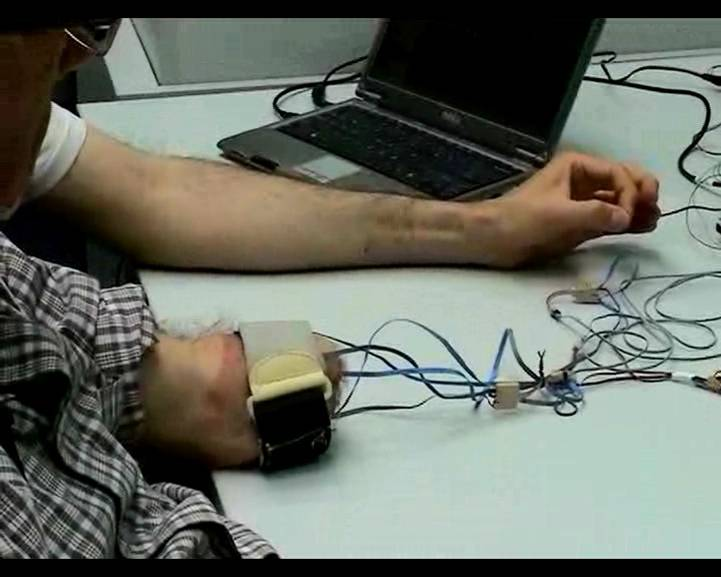
\includegraphics[width=0.3\textwidth]{figs/mod1} &
    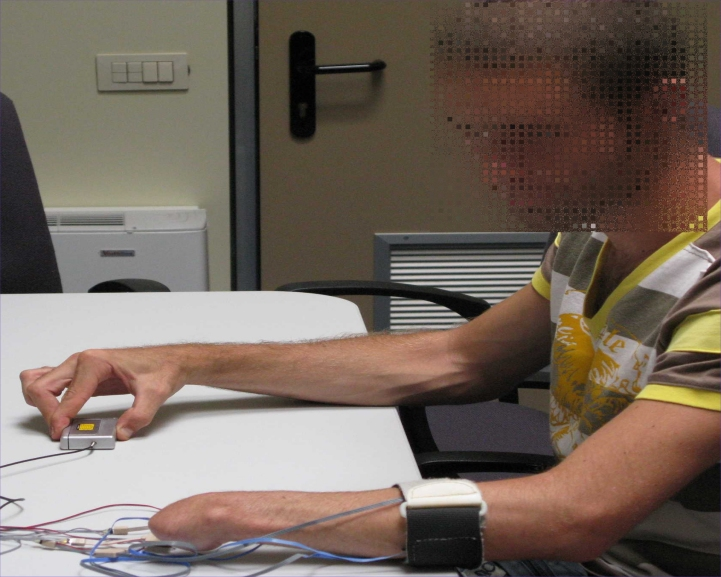
\includegraphics[width=0.3\textwidth]{figs/mod2} &
    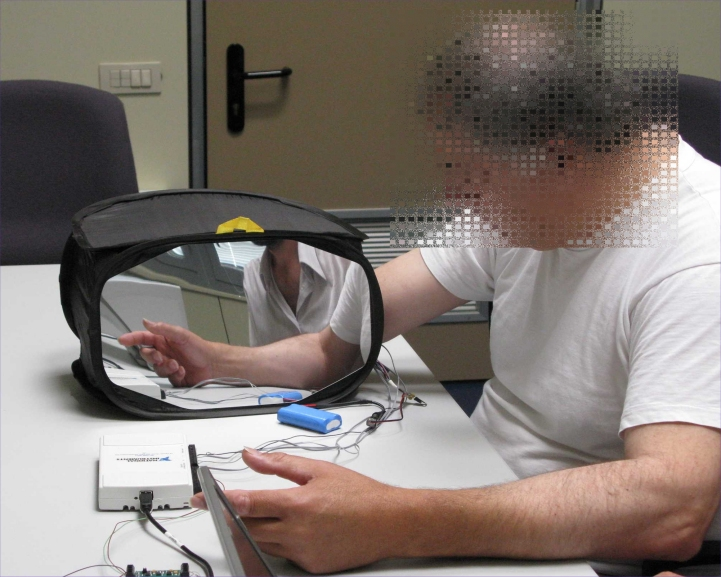
\includegraphics[width=0.3\textwidth]{figs/mod3} \\
    teacher imitation & bilateral action & mirror-box \\
  \end{tabular}
  \caption{the three training modalities.}
  \label{fig:modalities}
\end{figure*}

The patients were left free, to a large extent, to exert the postures
/ grips with the amount of force and the speed they liked; in some
phases of the experiment, the teacher would command them to grip
faster or slower, or with a certain desired force. The result is that
the patients applied a wide range of gripping speeds and forces, which
helped test whether our approach would work equally well with signals
gifted with diverse frequency and amplitude components. Figure
\ref{fig:ex_signals} shows some sample force and EMG signals. On
average, each modality lasted something more than $5$ minutes and no
subjects reported fatigue or pain. At the aforementioned sampling rate
of $100$Hz, we gathered a total of about $1.8$ million samples.

\begin{figure*}[!ht] \centering
  \begin{tabular}{ccc}
    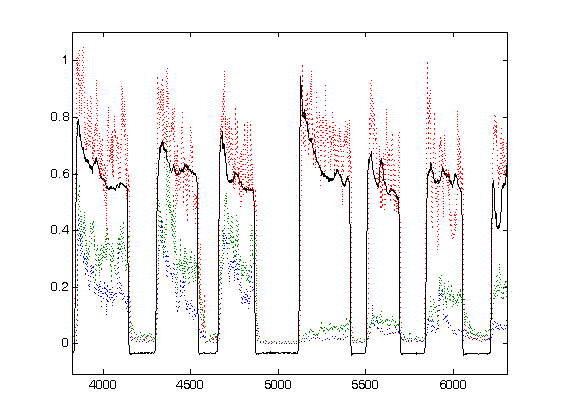
\includegraphics[width=0.3\textwidth]{figs/example_signal1} &
    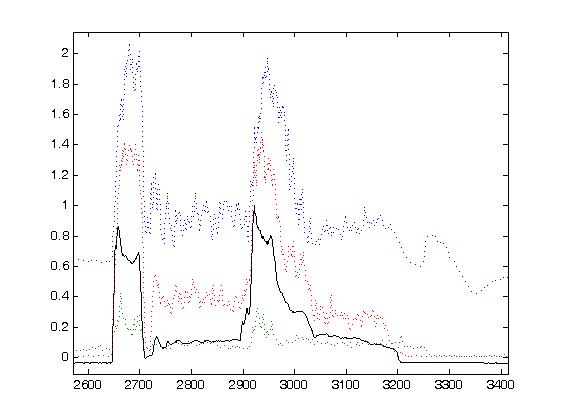
\includegraphics[width=0.3\textwidth]{figs/example_signal2} &
    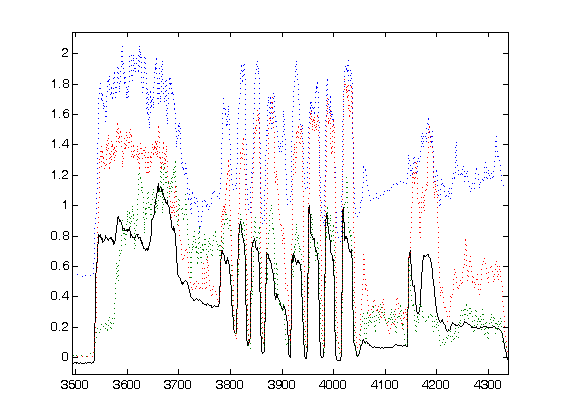
\includegraphics[width=0.3\textwidth]{figs/example_signal3} \\
  \end{tabular}
  \caption{three examples of force (black, continuous line) and EMG
    signals (coloured and dotted lines) during subjects'
    activity. (left panel) Modality $1$: around the $5000$th sample a
    switch from pointing index to  power grasp appears --- notice the
    related change in magnitude of the EMG. (center
    and right panels) Modality $3$, slow and fast power grasping ---
    notice two EMG electrodes spoiled by a non-null baseline and a
    slow drifting component, which was later on determined to be due
    to sweat.}
  \label{fig:ex_signals}
\end{figure*}

\subsection{Methods}

As already pointed out in literature, Support Vector Machines (SVM)
\cite{BGV92} are a good machine learning method for this framework, so we
employed them. For an explanation of how SVMs work in the context of
EMG signals, please refer to, among others,
\cite{2008.ICRA,2008.BioCyb}, whereas, for a comprehensive tutorial on
SVMs in the more general framework of classification and regression,
refer to \cite{Burges98,SmolaTut2004}. SVMs are a statistical learning
method able to build an approximated map between an input space and a
label (classification) or a real value (regression). Classification is
here used to classify the type of grasp according to the EMG signal,
whereas regression is used to understand how much force the subject is
exerting, independently from the grasp type.

The input space is chosen to be $\RR^5$, one coordinate for each EMG
electrode; the labels are five integer numbers, one for each grasp
type (six for subject $3$, who also performed the hand stretching
posture); and the real value is exactly the force value read off the
force sensor. Notice that we work in real-time, that is, our machines
associate a grasp type and a force value to an EMG value at each
instant of time. This approach enables us to detect a grasp type
almost at the onset of the grasping movement.
